\section{Lichtbrechung mittels Euler-Lagrange Gleichung}
\subsection{Einleitung}
Einige Optimierungsprobleme lassen sich direkt l"osen, indem sie in die
hergeleitete Euler-Lagrange-Gleichung eingesetzt werden k"onnen. Andere
Optimierungsprobleme, bei denen eine optimale Funktion gesucht
wird, k"onnen gel"ost werden indem sie das Prinzip der Variation der
Euler-Lagrange-Gleichung benutzen. Dazu reicht jedoch nicht mehr ein
\index{Euler-Lagrange-Gleichung}
einfaches einsetzen, sondern es muss eine neue Gleichung hergeleitet
werden. Die gesuchte Funktion wird dann gefunden, indem f"ur $g(y)$ und
$g'(y)$ konkret $y(x)$ und $y'(x)$ eingesetzt wird. Aber dazu sp"ater
noch mehr.

\subsection{Motivation f"ur die Variationsrechnung}
In \secref{brechungsgesetz} werden einfach geometrische Zusammenh"ange
hergeleitet, wenn zwei verschiedene benachbarte Medien einen
unterschiedlichen Brechungsindex haben. Komplexere Probleme k"onnen mit
diesen "Uberlegungen nicht mehr gel"ost werden. Der Unterschied liegt
darin, dass der Brechungsindex sich kontinuierlich im Raum "andert. In
einem  beliebigen  Medium  ist  der Brechungsindex variabel, eine
Funktion $n(x,y)$. Das  Problem wird erst mal nur 2-Dimensional
betrachtet. Mit diesen Begebenheiten ist es nicht mehr m"oglich, eine
einfache geometrische "Uberlegung  zur  Bestimmung  des  Strahles  zu
verwenden. der Lichtstrahl wird im allgemeinen gekr"ummt sein.

\subsection{Beschreibung einer Fata Morgana}
\index{Fata Morgana}
Bei der physikalischen Betrachtung der Lichtausbreitung wird davon
ausgegangen, dass sich Licht in
geradlinig verlaufenden Strahlen fortpflanzt. Das Auge erwartet das
Objekt, von dem die Lichtstrahlen
kommen in r"uckw"artiger geradliniger Verl"angerung der Richtung, welche
das Licht beim eintreffen in das Auge besitzt.
Wenn das Licht ein Medium, z.B. mit unterschiedlichen
Brechungsindizes durchquert, "andert es seine Richtung, siehe
\secref{brechungsgesetz}. Dies erkl"art z.B. die verk"urzten Beinen im
Schwimmbad.
Eine kompliziertere Situation liegt vor, wenn der Brechungsindex des
durchstrahlten Mediums kontinuierlich variiert. 
Dies ist der Fall, wenn die Luft in der N"ahe eines stark aufgeheizten
Untergrundes erw"armt
wird und infolge der dadurch bewirkten Dichte"anderung einen r"aumlichen
variierenden Brechungsindex annimmt. 
Das Licht "andert stetig seine Richtung, dass f"uhrt zu Ph"anomenen wie
Luftspiegelungen von Autolichtern oder einer Fata Morgana an heissen
Tagen \cite{fataEinleitung}.
In \figref{Ab:fataEinleitung} wird die Wahrnehmung des Auges und eine
Richtungs"anderung des Lichtes gezeigt.
\begin{figure}
\begin{center}
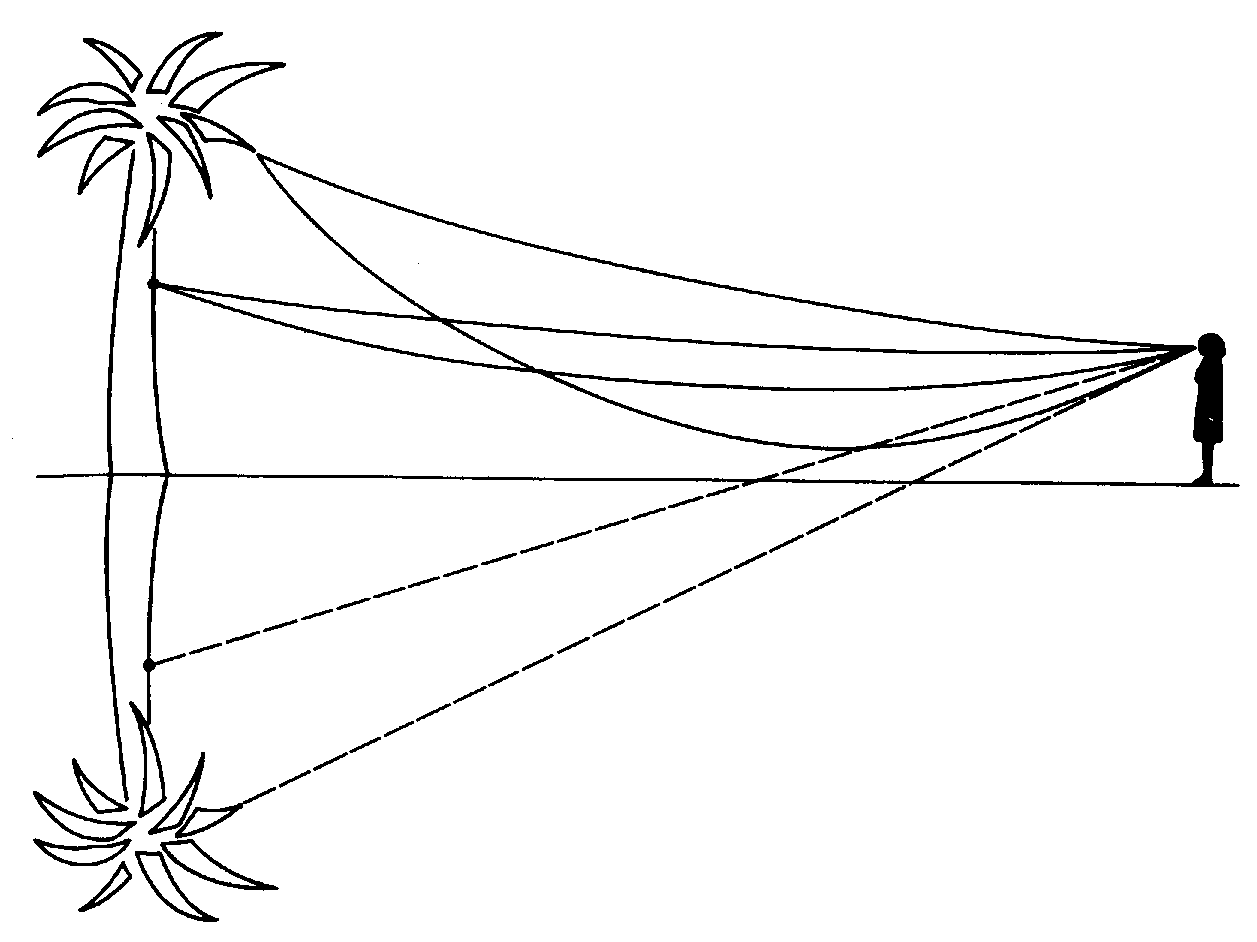
\includegraphics[width=0.55\textwidth]{licht/picture/FataEinleitung.png}
	\caption{Das Auge interpretiert, dass die Lichtstrahlen mit ver"anderter Richtung aus der tangentialen Verl"angerung kommen und sieht dort das Bild}
	\label{Ab:fataEinleitung}
\end{center}	
\end{figure}
\subsection{Untersuchung der Kr"ummungs-Eigenschaften bei einer
r"aumlichen Dichte"anderung \label{sec:Krummung}}
Bei einer Fata Morgana hat die Luft eine optische Dichte von $n(x,y)$. 
Dabei bewegt sich das Licht mit der Geschwindigkeit $c/n(x,y)$. 
Die ben"otigte Zeit, damit das Licht vom Punkt $(x_0, y_0)$ nach $(x_1,
y_1)$ braucht,
kann mit dem Kurvenintegral berechnet werden (\eqref{funktionTy}).
\begin{equation}
	T(y) = \int \limits_{x_0}^{x_1} \frac{n(x,y)}{c} \sqrt{1 + y'(x)^2} dx
	\label{funktionTy}
\end{equation}
Wie es bei einem heissen Tag auf einer Strasse oder in einer W"uste zutrifft,
nehmen wir zuerst nur einmal an, dass die optische Dicht nur von $y$
abh"angt und mit zunehmenden $y$ zunimmt,
$n(x,y) \rightarrow n(y)=g(y)$.
Durch die geringe Kr"ummung der Erde kann die $x$ Richtung vernachl"assigt
werden.
Dies bedeutet f"ur die Funktion $g(y)$, dass $g(y) > 0$ und $g'(y) > 0 $ ist.
Um dieses Minimalproblem zu l"osen, wird die allgemeine
Euler-Lagrange-Gleichung \chapref{chapter-variationsrechnung}
\eqref{variation:euler-gleichung}  aufgestellt. (\eqref{krummung})
ist somit unser vereinfachtes Funktional welches nur noch von $n(y)$
abh"angt.
\begin{equation}
	T(y) = \int \limits_{x_0}^{x_1} \frac{g(y)}{c} \sqrt{1 + y'(x)^2} dx = \frac{1}{c} \int \limits_{x_0}^{x_1} g(y) \sqrt{1 + y'(x)^2} dx
	\label{krummung}
\end{equation}
Der Faktor $\frac{1}{c}$ hat keinen Einfluss auf das Integral und somit
auch nicht auf das Variationsproblem. Deshalb kann er weggelassen werden,
um ihn nicht st"andig mitschleppen zu m"ussen.
Es werden nun die Ableitungen der Funktion \ref{funktionRech}
gebraucht. Sie sind in \ref{ableitungenLag} aufgef"uhrt.
\begin{align}
	F(x,y,y') &= g(y) \sqrt{1 + y'^2} \label{funktionRech} \\
	\frac{\partial F}{\partial y} &= g'(y) \sqrt{1 + y'^2} \notag \\
	\frac{\partial F}{\partial y'} &= g(y) \frac{y'}{\sqrt{1 + y'^2}} \label{ableitungenLag}
\end{align}
F"ur die Euler-Lagrange-Gleichung muss man im zweiten Ausdruck f"ur $y$
und $y'$ die Funktionen $y(x)$ 
sowie $y'(x)$ einsetzen und nach $\frac{d}{dx}$ ableiten, (\eqref{lagrange1}).
\begin{align}
	\frac{d}{dx} \frac{\partial F}{\partial y'} &= \frac{d}{dx} (g(y(x)) \frac{y'(x)}{\sqrt{1 + y'(x)^2}}) \notag \\ 
	&= g'(y(x)) \frac{y'(x)^2}{\sqrt{1 + y'(x)^2}} + g(y(x)) \frac{y''(x)}{\sqrt{1 + y'(x)^2}}
	 - g'(y(x)) \frac{y'(x)^2 y''(x)}{(1 + y'(x))^\frac{3}{2}} 
	 \label{lagrange1}
\end{align}
Auch im zweiten Term der Euler-Lagrange-Gleichung wird f"ur $y'$, $y'(x)$
eingesetzt. Es ergibt sich \eqref{lagrange2}
\begin{align}
	0 &= \frac{d}{dx} \frac{\partial F}{\partial y'} - \frac{\partial F}{\partial y} \label{lagrangePrinzip} \\
		0 &= \frac{d}{dx} \frac{\partial F}{\partial y'} - \frac{\partial F}{\partial y}
	= g'(y(x)) \frac{y'(x)^2}{\sqrt{1 + y'(x)^2}} + g(y(x)) \frac{y''(x)}{\sqrt{1 + y'(x)^2}} \notag \\
	&- g'(y(x)) \frac{y'(x)^2 y''(x)}{(1 + y'(x)^2)^\frac{3}{2}}  - g'(y(x)) \sqrt{1 + y'(x)^2}
	\label{lagrange2}
\end{align}
Da $\sqrt{1 + y'(x)^2} > 0$ und somit nicht gleich Null ist kann die
Gleichung mit $\sqrt{1 + y'(x)^2}$  multipliziert werden um einen
einfacheren Ausdruck zu bekommen, (\eqref{lagrange3}).
\begin{align}
	0 = g'(y(x)) y'(x)^2 + g(y(x)) y''(x) - g'(y(x)) \frac{y'(x)^2 y''(x)}{1 + y'(x)^2} - g'(y(x)) (1 + y'(x)^2)
	\label{lagrange3}
\end{align}
Auch $g(y(x))$ ist nicht gleich Null, da nach eingangs erfolgter
Definition $g(y(x)) > 0$, eine Division mit $g(y(x))$ ist somit zul"assig,
(\eqref{lagrange4}).
\begin{align}
	\frac{g'(y(x))}{g(y(x))} (1 + y'(x)^2) - \frac{g'(y(x))}{g(y(x))} y'(x)^2 &=  y''(x) - \frac{y'(x)^2 y''(x)}{1 + y'(x)^2} \notag \\
	\frac{g'(y(x))}{g(y(x))} (1 + y'(x)^2 - y'(x)^2) &= \frac{\left(1 + y'(x)^2 \right)y''(x) - y'(x)^2 y''(x)}{1 + y'(x)^2} \notag \\
	\frac{g'(y(x))}{g(y(x))} &= \frac{y''(x) + y'(x)^2 y''(x) - y'(x)^2 y''(x)}{1 + y'(x)^2} = \frac{y''(x)}{1 + y'(x)^2}\notag \\
	\frac{g'(y(x))}{g(y(x))} &= \frac{y''(x)}{1 + y'(x)^2}
	\label{lagrange4}
\end{align}
\eqref{lagrange4} kann jetzt auf ihre Eigenschaften bez"uglich der
Kr"ummung untersucht werden. Gem"ass den Definitionen von ganz am Anfang
ist die linke Seite positiv. 
Der Nenner der rechten Seite ist ebenfalls positiv. Daraus resultiert,
dass der Z"ahler der rechten Seite ebenfalls positiv sein muss
(\eqref{krummungAuswertung}).
\begin{align}
	\frac{g'(y(x))}{g(y(x))} > 0 \qquad \wedge \qquad (1 + y'(x)^2) > 0 \qquad \Rightarrow \qquad y''(x) > 0
	\label{krummungAuswertung}
\end{align}
Da die zweite Ableitung positiv ist, muss die Funktion des Lichtstrahles
konvex sein.
Dies bedeutet, dass der Lichtstrahl sich "uber dem Boden nach oben biegt,
ganz egal wie die Funktion von $g(x)$ aussieht, solange sie monoton
steigend ist.
Daraus kann die verallgemeinerte Schlussfolgerung gezogen werden, dass
der Lichtstrahl konkav sein muss, wenn die Funktion $g(x)$ monoton
fallend ist.
\begin{satz}
Ein Lichtstrahl wird in einem inhomogenen Medium in Richtung h"oherer
Dichte gekr"ummt, verh"alt sich die Dichte"anderung monoton fallend oder
steigend, nimmt der Lichtstrahl eine konvexe oder konkave Kurvenform an.
\index{Kr"ummung von Lichtstrahlen}
\end{satz}
\subsubsection{Technische Anwendung dieser Erkenntnis}
In einem Lichtwellenleiter wird dieses Ph"anomen ausgenutzt, 
indem  die  optische  Dichte  eines  zylindrischen
Lichtwellenleiters  von  der Achse zum Mantel hin abnimmt.
So werden die Lichtstrahlen immer vom Mantel weggekr"ummt 
und das Licht  bleibt im Leiter gefangen (\figref{lichtleiter}).
\begin{figure}
\begin{center}
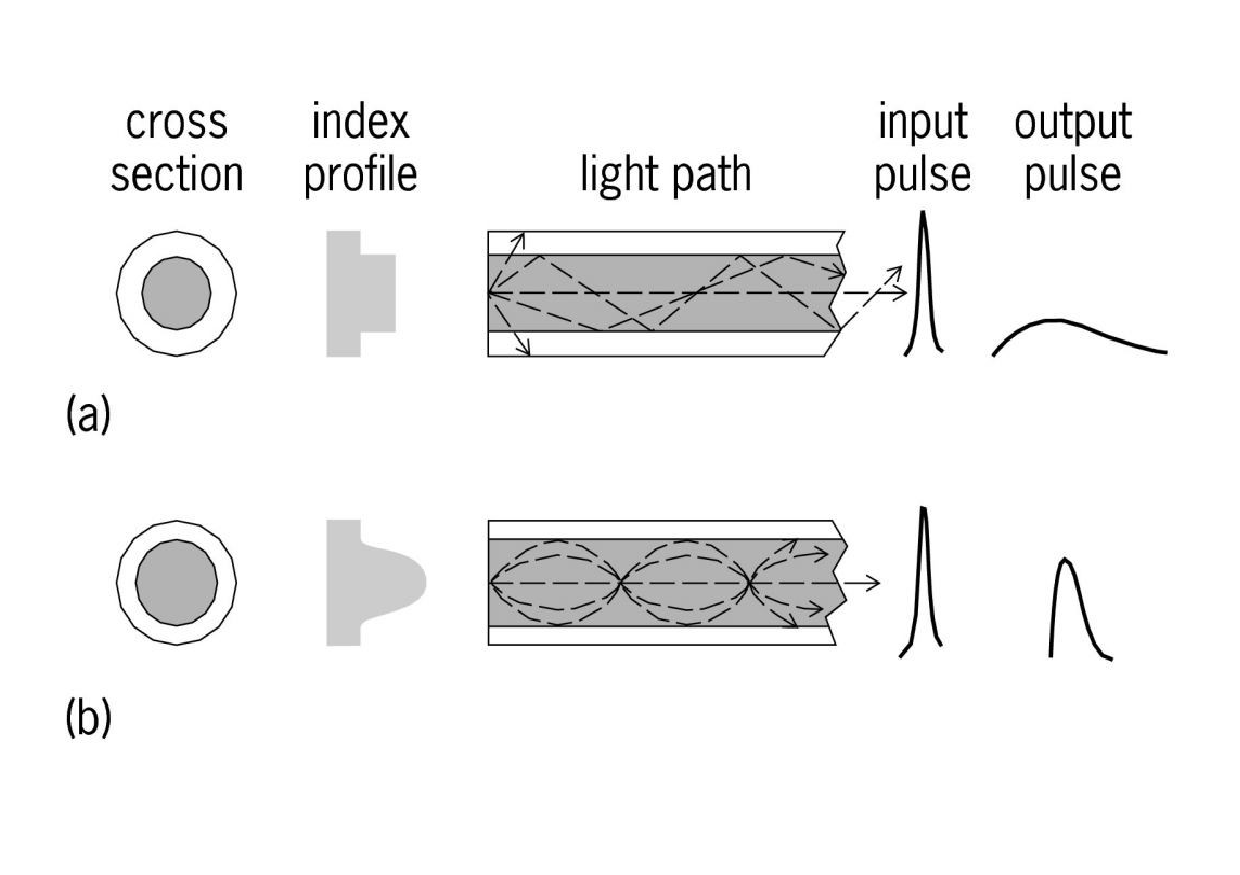
\includegraphics[width=0.5\textwidth]{licht/picture/Lichtwellenleiter.pdf}
	\caption{(a) Lichtwellenleiter mit einer Sprunghaften "Anderung der optischen Dichte erzeugt einen am "Ubergang reflektierenden Lichtweg. 
	(b) Lichtwellenleiter mit einer stetig "andernder optischer Dichte erzeugt einen kr"ummenden Lichtstrahl \cite{opticFibre}. }
	\label{lichtleiter}
\end{center}	
\end{figure}
\subsection{Berechnung der Differentialgleichung einer Fata Morgana \label{sec:diffgleichung}}
F"ur die gesuchte Differentialgleichung der Fata Morgana nehmen wir wie
bei der Kr"ummung an, dass die optische Dichtung nur von $y$ abh"angt
($n(y) = g(y)$) und mit zunehmenden $y$ zunimmt. Dies bedeutet, wie
f"ur die Funktion $g(y)$ wie in \secref{sec:Krummung}, dass $g(y) > 0$
und $g'(y) > 0 $ ist.
Die Euler-Lagrange-Gleichung wird gleich wie in \secref{sec:Krummung}
berechnet. Bei \eqref{lagrange4} wird weiter gerechnet. In
\eqref{diffgleichung1} werden alle Terme auf die linke Seite genommen.
\begin{align}
	g(y(x) y''(x)-g'(y(x) y'(x)^2 - g'(y(x)) =0 
	\label{diffgleichung1}
\end{align}
Dabei ist $g(y(x))$ die gesuchte Funktion des Brechungsindex $n(y)$. Mit
dieser Substitution ergibt sich die Differentialgleichung
\ref{diffgleichung2}.
\begin{align}
	n y''-n' (y')^2 - n' =0 
	\label{diffgleichung2}
\end{align}
In \secref{sec:Krummung} war anfangs definiert worden, dass die Dichte ab
dem Boden in Richtung $y$ zunimmt, weil die Temperatur "uber dem Boden von
dem heissen Untergrund mehr erhitzt ist als in h"oheren Lagen. Wird jetzt
diese Temperaturabnahme als linear angenommen, gilt \eqref{einsetzGl1}
und deren Ableitung \eqref{einsetzGl2}.
\begin{align}
	n(y)&=my+b \label{einsetzGl1} \\
	n'(y)&=m \label{einsetzGl2}
\end{align}
Um die Differentiation Gleichung zu l"osen, kann f"ur $y$ eine
hyperbolische Funktion \cite{cosh} gew"ahlt werden (\eqref{hyperFunk}).
\begin{align}
	y&=A\cosh(Bx+C)+D \label{hyperFunk} \\
	y'&= A B \sinh(B x + C) \label{hyperFunkDx} \\
	y''&= A B^2 \cosh(B x + C) \label{hyperFunkD2x}
\end{align}

\subsubsection{Eine Beispielaufgabe}
Folgende Annahmen gelten:
\begin{align}
	y_0&=y_1=2 m & \text{Augenh"ohe und Startpunkt} \notag \\
	-x_0&=x_1 = 200m & \text{Distanz zum Nullpunkt des Koordinatensystems} \notag \\
	T_A&=333.15 K & \text{Temperatur des Asphalt}  \notag \\
	T_L&=293.15 K & \text{Temperatur Luft auf Augenh"ohe}  \notag
\end{align}
Daraus ergeben sich mit \eqref{brechTemp} eine Funktion f"ur den
Brechungsindex von Luft in Abh"angigkeit von Temperatur.
\begin{align}
	n=1+0.000293\frac{T_0}{T}
	\label{brechTemp}
\end{align}
Daraus ergeben sich die Werte in \eqref{nParam} f"ur unsere lineare Gleichung
$n(y)=my+b$
\begin{align}
	y&=y_0=y_1 \notag \\
	b&=n_A=1+0.000293\frac{273.15 K}{333.15 K} = 1.00024 \notag \\
	n_L&=1+0.000293\frac{273.15 K}{293.15 K} = 1.00027 \notag \\
	m&=\frac{\delta n}{y}=\frac{n_L-n_A}{y}=1.64*10^{-5} \notag \\
	n(y)&=my+b=1.64*10^{-5}y +1.00024
	\label{nParam}
\end{align}
Als erstes die allgemeine Form mit einsetzen von $n,n',y',y''$
(\eqref{HauptGl}).
\begin{align}
	(my_0+b)A B^2 \cosh(B x_0 + C)-m (A B \sinh(B x_0 + C))^2-m &= 0\notag \\
	(my_1+b)A B^2 \cosh(B x_1 + C)-m (A B \sinh(B x_1 + C))^2-m &=0 \label{HauptGl}
\end{align}
Da wir mit $-x_0=x_1$ eine Achsenspiegelung haben und die Cosinus Hyperbolicus Funktion eine gerade Funktion ist, l"asst sich (\eqref{HauptGl}) vereinfachen (\eqref{glvereinfacht}). Dabei wird $C$ weggelassen.
\begin{align}
	(my_0+b)A B^2 \cosh(B x_0 )-m (A B \sinh(B x_0 ))^2-m &= 0\notag \\
	(my_1+b)A B^2 \cosh(B x_1 )-m (A B \sinh(B x_1 ))^2-m &=0 \label{glvereinfacht}
\end{align}

 \eqref{hyperFunk}
ist nicht linear, deshalb muss ab hier mit numerischen Methoden
weitergearbeitet werden.
 
 \subsection{Schlussfolgerungen}
Die Erkenntnis das f"ur $y$ eine Hyperbolische Funktion resultiert
und das eine Differentialgleichung f"ur beliebige Funktionen f"ur $n$
eingesetzt werden k"onnen ist beachtlich. Die Variationsrechnung
ist sehr m"achtig, es k"onnen allgemeine Eigenschaften die nicht
Funktionsabh"angig sind abgeleitet werden (\secref{sec:Krummung}). Es
k"onnen auch nicht triviale Differentialgleichungen hergeleitet werden
(\secref{sec:diffgleichung}). Wenn ein Problem nicht direkt mit der
Euler-Lagrange-Gleichung gel"ost werden kann, kann das Prinzip des etwas
''verwackeln'' und der Annahme, dass sich das Integral nicht "andert, oft
trotzdem angewendet werden. Es muss dann eine neue Gleichung hergeleitet
werden, welche danach wieder auf die Euler-Lagrange-Gleichung
zur"uckzuf"uhren ist (\chapref{chapter-variationsrechnung}
\eqref{variation:euler-gleichung}).
